\documentclass{article}
\usepackage{amsmath}
\usepackage{amssymb}
\usepackage{graphicx}
\usepackage{hyperref}
\usepackage[version=4]{mhchem}

\title{Example 7}
\date{}

\begin{document}
\maketitle

Given any \(\triangle A B C, A E\) bisects \(\angle B A C, B D\) bisects \(\angle A B C\), \(C P \perp B D\), and \(C Q \perp A E\), prove that \(P Q\) is parallel to \(A B\).

Solution:
Method 1:\\
\centering
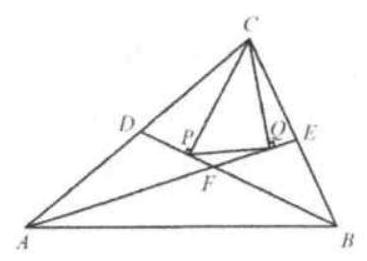
\includegraphics[width=\textwidth]{images/058(2).jpg}


Extend \(C P\) and \(C Q\) to meet \(A B\) at \(S\) and \(R\), respectively.\\
Since \(B P\) is the perpendicular bisector of \(C S\), and \(A Q\) is the perpendicular bisector of \(C R\), it shows that \(\triangle C P B \cong \triangle S P B\), and \(\triangle C Q A \cong \triangle R Q A\), respectively.\\
It then follows that \(C P=S P\) and \(C Q=R Q\) or \(P\) and \(Q\) are midpoints of \(C S\) and \(C R\), respectively. Therefore, in \(\triangle C S R, P Q / / S R\). Thus, \(P Q / / A B\).

Method 2:
\begin{center}
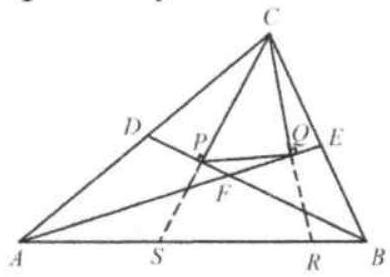
\includegraphics[width=\textwidth]{images/059(3).jpg}
\end{center}

Connect \(C F\). We know that \(C F\) bisects \(\angle A\).\\
Since \(\angle C P F=\angle C Q F=90^{\circ}, \mathrm{CPFQ}\) are concyclic.\\
Thus \(\angle P C F=\angle P Q F=\frac{\angle C}{2}-\angle P C D\)\\
\(=\frac{\angle C}{2}-(\angle C-\angle P C E)=\frac{\angle C}{2}-\left[\angle C-\left(90^{\circ}-\frac{\angle B}{2}\right)\right]\)\\
\centering
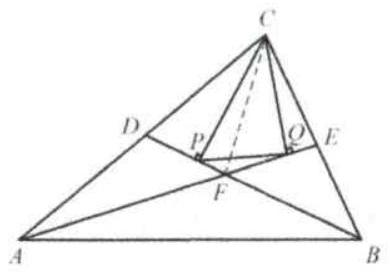
\includegraphics[width=\textwidth]{images/059(1).jpg}\\
\(=90^{\circ}-\frac{\angle C}{2}-\frac{\angle B}{2}=\frac{\angle B}{2}=\frac{180^{\circ}-\angle C-\angle B}{2}=\frac{\angle A}{2}=\angle E A B\).\\
Thus, \(P Q / / A B\).\\

\end{document}
